\begin{frame}{¿Qu\'e es este \textit{software}?}



    \begin{block}{Sistemas de gesti\'on de bases de datos (SGBD)}
        \begin{quote}
            ``Un \textcolor{red}{sistema de gesti\'on de bases de datos}
            es un sistema computacional que proporciona
            \textcolor{red}{funcionalidades, medios o servicios para manipular} y, en particular,
            \textcolor{red}{manejar todos los accesos} a una base de datos o una colecci\'on
            de bases de datos." \hspace{1em plus 1fill}---C. J. Date
        \end{quote}
    \end{block}
\end{frame}


\begin{frame}{Superando limitaciones}
       
            \begin{block}{}
                \begin{itemize}
                    \item<1-> \textbf{Persistencia}: los datos permanecen en memoria externa
                    \item<2-> \textbf{Masivos}: manejan terabytes/petabytes de datos
                    \item<3-> \textbf{Eficientes}: operaciones eficientes gracias al uso de estructuras de datos y algoritmos
                    \item<4-> \textbf{Multi-usuarios}: protocolos para la gesti\'on de accesos concurrentes
                    \item<5-> \textbf{Seguros}: consistentes ante accesos por usuarios no autorizados y fallos del sistema
                    \item<6-> \textbf{Confiables}: disponibles al 99.99999\%
                \end{itemize}
            \end{block}
               
\end{frame}


\begin{frame}{Superando expectativas}
    \begin{block}{Conveniencia de los SGBD}
        \begin{itemize}
            \item<2-> \textbf{Independencia f\'isica de datos}: admiten el cambio de la forma de
            almacenamiento de los datos, pero la estructura de la base de datos y las operaciones
            definidas sobre ella no cambian.
            \item<3-> \textbf{Independencia l\'ogica de datos}: proporcionan lenguajes de consulta declarativos, se define
            lo que se desea pero no c\'omo alcanzarlo.
        \end{itemize}
        
    \end{block}

\end{frame}


\begin{frame}{Superando las expectativas}
    \centering
    \begin{tikzpicture}
        \node at (1.4,7) {\tiny \bf {Usuario de SGBD}} ;
        \node[inner sep=0pt] at (1.4,5.8) {
            
\includegraphics[width=1.8cm]{img/hface.png}
        };

        \node at (1.4,4.3) {\tiny \bf {Desarrollador de SGBD}} ;
        \node[inner sep=0pt] at (1.4,3.2) {
            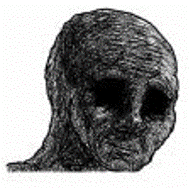
\includegraphics[width=1.8cm]{img/sface.png}
        };

        \draw[-,thick] (0.3, 4.6) -- (7,4.5);
        \draw[-,thick] (2.7, 2) -- (2.7,7.4);

        \node at (5,5.8) {Lenguaje declarativo};
        \node at (5,4.3) {Estructuras de datos};%\\Algoritmos\\Optimizaci\'on\\Compilaci\'on\\Gesti\'on de ficheros};
        \node at (5,3.8) {Algoritmos};%\\Algoritmos\\Optimizaci\'on\\Compilaci\'on\\Gesti\'on de ficheros};
        \node at (5,3.3) {Optimizaci\'on};%\\Algoritmos\\Optimizaci\'on\\Compilaci\'on\\Gesti\'on de ficheros};
        \node at (5,2.8) {Compilaci\'on};%\\Algoritmos\\Optimizaci\'on\\Compilaci\'on\\Gesti\'on de ficheros};
        \node at (5,2.3) {Gesti\'on de ficheros};%\\Algoritmos\\Optimizaci\'on\\Compilaci\'on\\Gesti\'on de ficheros};

    \end{tikzpicture}
\end{frame}